% DermaJEPA — preliminary report (v0.1 draft)
% Author: Abdelhamid Bakhta
% Build: make pdf
% Companion docs: ../docs/paper/{OUTLINE.md, WRITING-PLAN.md, REVIEWER-QA.md}

\documentclass[11pt,a4paper]{article}

% --- packages -----------------------------------------------------------------
\usepackage[utf8]{inputenc}
\usepackage[T1]{fontenc}
\usepackage{lmodern}
\usepackage{microtype}

\usepackage{amsmath, amssymb, amsthm}
\usepackage{graphicx}
\usepackage{booktabs}
\usepackage{siunitx}
\sisetup{detect-all=true, group-separator={,}, group-minimum-digits=4}
\usepackage{xcolor}
\usepackage{enumitem}
\setlist{noitemsep, topsep=2pt}
\usepackage[colorlinks=true, urlcolor=blue, citecolor=blue, linkcolor=black]{hyperref}
\usepackage{url}
\usepackage{geometry}
\geometry{margin=2.5cm}
\usepackage{authblk}

% Editorial todo notes; suppress at submission with \usepackage[disable]{todonotes}
\usepackage[textsize=small, color=yellow!40, bordercolor=yellow!70!black]{todonotes}

% --- metadata -----------------------------------------------------------------
\title{Frozen-backbone JEPA-style probes on HAM10000:\\
       preliminary results from a nine-experiment ablation,\\
       with an unpartitioned contamination caveat}
\author{Abdelhamid Bakhta}
\affil{\href{https://github.com/AbdelStark/derma-jepa}{github.com/AbdelStark/derma-jepa}}
\date{Preliminary report --- 2026}

% --- macros -------------------------------------------------------------------
\newcommand{\auroc}{\mathrm{AUROC}}
\newcommand{\strongfam}{\texttt{strong}}
\newcommand{\strongholdone}{\texttt{strong\_held\_out}}
\newcommand{\strongholdtwo}{\texttt{strong\_held\_out\_2}}
\newcommand{\runarchive}{\href{https://huggingface.co/datasets/abdelstark/derma-jepa-runs}{\texttt{abdelstark/derma-jepa-runs}}}

% --- document -----------------------------------------------------------------
\begin{document}
\maketitle

\begin{abstract}
Self-supervised representations promise robustness to nuisance variation; whether
that robustness transfers across novel nuisance families is rarely tested. We
probe this on a leakage-controlled HAM10000 longitudinal proxy with three
disjoint synthetic nuisance families --- partitioned along the deterministic-
augmentation axis --- training a JEPA-style latent predictor on stable pairs
from two of three families and evaluating on the third unseen family. We report
a preliminary nine-experiment arc. Across four frozen-natural-image
configurations spanning two pretraining paradigms within the ViT-B
class (DINOv2 ViT-B/14, OpenAI CLIP ViT-B/16), two predictor
scaffolds (linear with identity warm-start, 2-layer identity-residual
MLP), and two optimisers (SGD, Adam), test $\auroc$ on the held-out
family lands in $0.25$--$0.29$ --- below random and below the
strongest oriented baseline (pixel L2 at $0.580$). A frozen general-medical
backbone (BiomedCLIP, PMC-15M scientific-article figures, with no
documented raw HAM10000/ISIC archive ingestion) lifts test $\auroc$ by
only $+0.04$ to $0.329 \pm 0.012$ across $5$ seeds. A frozen
dermoscopy-pretrained backbone
(DermLIP, Derm1M) lifts test $\auroc$ to $\mathbf{0.944 \pm 0.003}$ across $5$
seeds, $+0.363$ above the strongest baseline and the only above-random result on
the held-out third family across the six runs that evaluate on it
(EXP-004 through EXP-008). Holding architecture (ViT-B/16) and
predictor (linear) constant, varying only the pretraining-data domain
produces a $+0.66$ end-to-end $\auroc$ swing (web $\to$ dermoscopy)
that is concentrated in the dermoscopy-specific step ($+0.62$ of $+0.66$,
with the residual $+0.04$ at the web $\to$ general-medical step).
\textbf{We explicitly do not claim that this swing is dermoscopy-domain
transfer}: DermLIP's Derm1M corpus does not list HAM10000 as a source, but a
perceptual-hash audit confirms HAM10000 images leaked into it via reproduced
figures in its scraped literature, so image-level overlap is established (at
small, lower-bounded scale), and the experiments reported here cannot separate
dermoscopy-domain transfer from such overlap. We release the methodology, the configurations,
and the run archive, and sketch a candidate partition experiment (a
non-HAM10000 dermoscopy SSL pretrain) as a natural next step we may
consider after gathering community feedback on the methodology and the
preliminary results. The contribution is the
proxy-task design, the failure characterisation, and a clearly scoped open
question --- not a conclusion about whether frozen-backbone JEPA generalises on
dermoscopy.

\end{abstract}

\section{Introduction}
\label{sec:introduction}

Lesion monitoring is fundamentally a change-detection problem under heavy
nuisance variation. Repeated photographs of the same skin lesion vary because
of illumination, framing, hair occlusion, camera optics, and compression;
clinically meaningful change is small relative to that nuisance envelope.
Self-supervised representations are pitched as nuisance-invariant
\citep{caron2021dino, oquab2024dinov2, radford2021clip}, with the JEPA family
\citep{lecun2022path, assran2023ijepa} explicitly framing prediction in
representation space as the path to invariance. Our question is narrow:
\emph{when a JEPA-style latent predictor over a frozen vision backbone is
trained on stable-pair invariance with respect to one set of synthetic nuisance
operations, does that invariance generalise to a disjoint nuisance family the
predictor never saw at training time?}

We probe this on HAM10000 \citep{tschandl2018ham10000}. HAM10000 is
cross-sectional, so we construct a leakage-controlled longitudinal proxy:
lesion-ID-aware splits, synthetic stable-pair augmentations applied
post-split, and changing-pair construction matched on diagnosis and anatomical
site. Three deterministic synthetic nuisance families --- \strongfam,
\strongholdone, and \strongholdtwo\ --- are designed to share no operation
type with each other. We train on stable pairs drawn from $\{\strongfam,
\strongholdone\}$ and evaluate on a third unseen family $\strongholdtwo$. The
predictor is a small function $g_\theta : \mathbb{R}^d \to \mathbb{R}^d$ over
the L2-normalised output of a frozen backbone --- linear with identity
warm-start, or a 2-layer identity-residual MLP --- trained to minimise L2-MSE
between predicted and observed target latents on stable pairs. Across nine
experiments we vary predictor class, optimiser, and backbone independently
while holding every other knob constant.

\textbf{This paper is a preliminary report.} The single positive result we
observe (frozen DermLIP at $0.944 \pm 0.003$ test $\auroc$ across $5$ seeds)
\emph{cannot be attributed to dermoscopy-domain transfer with the experiments
reported here.} DermLIP's pretraining corpus, Derm1M
\citep{yan2025derm1m}, almost certainly contains HAM10000 raw images, and the
BiomedCLIP partition we report rules out only the broader ``any medical-image
pretraining is sufficient'' alternative. EXP-009 (a self-pretrained DINOv2 on a
non-HAM10000 dermoscopy corpus, see \S\ref{sec:followup}) is the experiment
that would close the partition. Building that corpus is multi-week work; we
share the methodology and the nine-run arc at this stage to validate the proxy
design and to invite feedback on the partition before committing to it.

Figure~\ref{fig:cross-backbone-gradient} previews the headline. Test $\auroc$
on $\strongholdtwo$ is below random for every frozen natural-image backbone
across two architectures and three predictor scaffolds; barely lifts under a
frozen general-medical backbone (BiomedCLIP, $0.329 \pm 0.012$); and reaches
$0.944 \pm 0.003$ under a frozen dermoscopy-specific backbone (DermLIP), with
the contamination caveat marked on the right.

\paragraph{Contributions.}
\begin{itemize}
\item \textbf{Methodological.} A leakage-controlled HAM10000 longitudinal-proxy
      task with three disjoint synthetic nuisance families and a
      \texttt{train-on-two/evaluate-on-third} protocol, released as code,
      configurations, and reproduction launchers.
\item \textbf{Empirical (negative).} Across two architectures, three
      predictor scaffolds, and two optimisers, frozen natural-image backbones
      produce below-random inverted test $\auroc$ on the held-out third
      family.
\item \textbf{Empirical (positive but unpartitioned).} Frozen DermLIP reaches
      test $\auroc = 0.944 \pm 0.003$ across $5$ seeds, $+0.364$ above the
      strongest baseline. The win cannot yet be attributed to dermoscopy-
      domain transfer rather than HAM10000 image-level overlap; EXP-009
      (\S\ref{sec:followup}) is the open partition.
\item \textbf{Empirical (negative-as-partition).} Frozen BiomedCLIP --- the
      cleanest publicly available ``general medical pretraining without
      HAM10000'' backbone --- lifts only $+0.04$ over web CLIP, ruling out
      ``any medical-image pretraining'' as sufficient.
\item \textbf{Reproducibility.} Every primary-tier run is archived publicly at
      \runarchive\ with manifests, embeddings, metrics, model card, and logs.
      A single launcher script reproduces each run end-to-end on a free A10G
      via Hugging Face Jobs.
\item \textbf{A clearly-scoped open question.} The EXP-009 design and decision
      table are stated up front (\S\ref{sec:followup}) rather than treated as
      future work in passing.
\end{itemize}

\section{Related work}
\label{sec:related-work}

\paragraph{JEPA-style and self-supervised image representations.}
The Joint-Embedding Predictive Architecture family
\citep{lecun2022path, assran2023ijepa} predicts in representation space rather
than pixel space, motivated by the conjecture that nuisance-invariant
representations emerge from learning to predict the latents of related views.
DINO \citep{caron2021dino} and DINOv2 \citep{oquab2024dinov2} train
transformers via self-distillation to produce features that transfer
across image distributions and downstream tasks; CLIP
\citep{radford2021clip} and OpenCLIP \citep{cherti2023openclip} build
transferable representations via contrastive image--text alignment;
MAE \citep{he2022mae} reconstructs masked pixels and VICReg
\citep{bardes2022vicreg} regularises variance, invariance, and
covariance of the embedding. We read all of these as different routes
toward representations that are approximately invariant to many
photometric and framing nuisances; our probe asks whether that
invariance generalises to nuisance families held out from the probe's
training distribution. Our probe is
narrow: the frozen-backbone, single-step, stable-pair subset of the JEPA family
applied as an evaluation probe, not a pretraining objective.

\paragraph{Domain-specific medical foundation models.}
BiomedCLIP \citep{zhang2023biomedclip} is a CLIP-style model trained on
PMC-15M, $\sim$$15$\,M biomedical image--text pairs from $\sim$$4.4$\,M
scientific articles. DermLIP \citep{yan2025derm1m} is a CLIP-style model trained on
Derm1M, a $\sim$1 million dermatology image--text corpus that aggregates
publicly available dermoscopy datasets and dermatology-website content.
A broader dermatology foundation-model line includes MONET
\citep{kim2024monet} (image--text alignment over dermatology textbook
figures and PubMed) and PanDerm \citep{yan2024panderm} (a multi-modal
self-supervised model trained on $\sim$$2$M dermatology images);
RETFound \citep{zhou2023retfound} is a comparable medical-domain
foundation-model precedent in retinal imaging, cited here for the
domain-specific FM design pattern rather than as a methodological
template for our probe. We use BiomedCLIP and DermLIP as third-party frozen weights,
not as artefacts to evaluate in their own right; the paper makes no
claim about either model beyond the test $\auroc$ each produces under
our specific probe.

\paragraph{Distribution-shift evaluation.}
WILDS \citep{koh2021wilds} and the in-search-of-lost-DG framing
\citep{gulrajani2021dg} establish the modern protocol for distribution-shift
evaluation. Our contribution is complementary: a deterministic, leakage-
controlled, three-family-disjoint nuisance design that lets the experimenter
precisely control the operation-level overlap between train and test nuisance.
Where WILDS varies natural distributions (hospital, scanner, country), we vary
synthetic nuisance families partitioned along the augmentation axis. The two
designs answer different questions; the methodology proposed here is most
useful when the natural axis of variation is hard to disentangle from the
target signal, as in dermoscopic re-photography. ISIC challenge artefacts
\citep{codella2018isic, combalia2019bcn20000} provide additional dermoscopy
corpora that remain unprobed in this work and are candidates for the EXP-009
partition pretraining set (\S\ref{sec:followup}).

\section{Method}
\label{sec:method}

\subsection{Notation and probe}
\label{sec:method:notation}

Let $f : \mathcal{X} \to \mathbb{R}^{d}$ be a frozen vision encoder with
output dimension $d$, and define the L2-normalised representation
\begin{equation}
  z(x) \;=\; \frac{f(x)}{\lVert f(x) \rVert_{2}} \;\in\; \mathbb{S}^{d-1}.
\end{equation}
A \emph{stable} pair $(x_{c}, x_{t})$ shares a single underlying lesion image
$u$ subjected to two independent draws of a synthetic nuisance augmentation
$\nu \sim \mathcal{N}_{F}$ from family $F$:
\begin{equation}
  x_{c} = \nu_{c}(u), \qquad x_{t} = \nu_{t}(u), \qquad \nu_{c}, \nu_{t} \sim \mathcal{N}_{F}.
\end{equation}
A \emph{changing} pair pairs two distinct lesions $u_{1}, u_{2}$ matched on
diagnosis $\mathrm{dx}(u_{1}) = \mathrm{dx}(u_{2})$ and anatomical site
$\mathrm{site}(u_{1}) = \mathrm{site}(u_{2})$; each side receives an
independent nuisance draw. The predictor $g_{\theta} : \mathbb{R}^{d} \to
\mathbb{R}^{d}$ minimises the L2-MSE objective on stable training pairs:
\begin{equation}
  \mathcal{L}(\theta) \;=\; \frac{1}{|\mathcal{D}_{\mathrm{train}}^{\mathrm{stable}}|}\!\!
  \sum_{(x_{c}, x_{t}) \in \mathcal{D}_{\mathrm{train}}^{\mathrm{stable}}}
  \lVert g_{\theta}(z(x_{c})) - z(x_{t}) \rVert_{2}^{2}
  \;+\; \mathcal{R}(\theta),
  \label{eq:loss}
\end{equation}
where $\mathcal{R}$ is a predictor-specific regulariser. For the linear
predictor we use a soft \texttt{weight $-$ I} penalty,
$\mathcal{R}(\theta) = \lambda \, \lVert W - I \rVert_{F}^{2}$, which, in
combination with the identity warm-start ($W \approx I$ at step zero,
\S\ref{sec:method:predictor}), holds the function near the identity at
initialisation. For the 2-layer identity-residual MLP, the residual
weight $W_{2}$ is zero-initialised so the predictor is identity at step
zero by construction, and $\mathcal{R}$ is standard $L^{2}$ weight decay
on the predictor weights (decoupled, in the Adam configuration);
applying a $\lVert W_{2} - I \rVert_{F}^{2}$ penalty here would
contradict the zero-init identity warm-start. Per-variant values of
$\lambda$ are listed in Appendix~\ref{app:hyperparameters}. At
evaluation time, the score for a
pair is the cosine \emph{distance} between the L2-normalised prediction and
the L2-normalised target:
\begin{equation}
  s(x_{c}, x_{t}) \;=\; 1 \;-\; \langle \tilde{g}_{\theta}(z(x_{c})), z(x_{t}) \rangle, \qquad
  \tilde{g}_{\theta}(\cdot) := \frac{g_{\theta}(\cdot)}{\lVert g_{\theta}(\cdot) \rVert_{2}}.
  \label{eq:score}
\end{equation}
A correctly oriented predictor produces $s(x_{c}, x_{t}) < s(x_{c}', x_{t}')$
whenever $(x_{c}, x_{t})$ is stable and $(x_{c}', x_{t}')$ is changing;
$\auroc$ quantifies this ranking.

\subsection{Predictor variants}
\label{sec:method:predictor}

\paragraph{Linear with identity warm-start.}
$g_{\theta}(z) = W z + b$ with $W$ initialised to $I + \epsilon$,
$\epsilon_{ij} \overset{\text{iid}}{\sim} \mathcal{N}(0, 0.005^{2})$, and
$b = 0$. Under SGD with the soft \texttt{weight $-$ I} penalty above, the
predictor at step zero is identity-equivalent.

\paragraph{2-layer identity-residual MLP.}
$g_{\theta}(z) = z + W_{2} \,\mathrm{ReLU}(W_{1} z + b_{1}) + b_{2}$, with
$W_{2}$ zero-initialised so the residual term vanishes at step zero and
$g_{\theta} = \mathrm{identity}$. Hidden dimension $512$.

\subsection{Three nuisance families}
\label{sec:method:nuisance}

The augmentation suite specifies three deterministic synthetic nuisance
families, summarised in Table~\ref{tab:nuisance-families}. The disjointness
rule is operation-level: no transform type is shared between any two
families. The exact operation parameters are listed in
Appendix~\ref{app:nuisance-operations}.

\begin{table}[h]
\centering
\small
\begin{tabular}{@{}lp{0.65\linewidth}@{}}
\toprule
Family & Operation set \\
\midrule
\strongfam            & brightness $\times$ contrast $\times$ saturation, rotation $\pm 15^{\circ}$, scale $0.82$--$1.00$, translate $\pm 5\%$, horizontal flip, Gaussian blur, Gaussian noise, JPEG quality $45$--$70$ \\
\strongholdone        & hue shift $\pm 12^{\circ}$ (HSV rotation), posterise $4$--$6$ bits, unsharp-mask sharpen, motion blur (linear kernel $5$--$15$\,px), random rectangular erasing $6$--$18\%$ area, JPEG quality $20$--$40$ \\
\strongholdtwo        & gamma $0.6$--$1.6$, colour temperature $0.85$--$1.15$, radial vignette $25$--$55\%$ falloff, salt-and-pepper noise $0.5$--$2.5\%$, JPEG quality $80$--$95$ \\
\bottomrule
\end{tabular}
\caption{Three deterministic nuisance families, partitioned along the
operation axis. Train stable pairs draw from $\{\strongfam, \strongholdone\}$;
val and test stable pairs use $\strongholdtwo$.}
\label{tab:nuisance-families}
\end{table}

\subsection{Splits and pair construction}
\label{sec:method:splits}

We use lesion-ID-aware splits at fractions $0.70 / 0.15 / 0.15$, deterministic
from a fixed seed, with group counts $5{,}229 / 1{,}120 / 1{,}121$ across
HAM10000's $10{,}015$ images and $7{,}470$ unique lesions. Each split
contains $1{,}000$ stable plus $1{,}000$ changing pairs (total $6{,}000$
pairs per run). The strict same-diagnosis-site changing-pair policy requires
that a context lesion's changing partner be a distinct lesion with identical
diagnosis and identical anatomical site. Train stable pairs rotate
deterministically between \strongfam\ and \strongholdone\ by pair index; val
and test stable pairs use \strongholdtwo\ exclusively.

\subsection{Evaluation protocol}
\label{sec:method:eval}

We report $\auroc$ as the primary metric, with $1{,}000$-sample bootstrap
$95\%$ confidence intervals computed by per-pair resampling. AUPRC, equal-
error-rate threshold, and FPR at fixed TPR $= 0.8$ accompany every run, as do
three representation-health checks: prediction-norm mean and minimum,
dimension-variance mean and minimum, and a binary \texttt{collapsed} flag
triggered when either falls below $10^{-8}$. None of the nine reported runs
is flagged as collapsed.

\section{Experimental setup}
\label{sec:experimental-setup}

\paragraph{Backbones.} Five frozen vision backbones cover the
architectural and pretraining-data axes the paper varies
(Table~\ref{tab:backbones}).

\begin{table}[h]
\centering
\footnotesize
\setlength{\tabcolsep}{4pt}
\begin{tabular}{@{}llrlp{0.36\linewidth}@{}}
\toprule
Backbone & Arch. & $d$ & Pretraining & Hugging Face Hub path \\
\midrule
DINOv2 ViT-S/14      & ViT-S/14 & $384$ & LVD-142M (web)   & \path{facebook/dinov2-small} \\
DINOv2 ViT-B/14      & ViT-B/14 & $768$ & LVD-142M (web)   & \path{facebook/dinov2-base} \\
OpenAI CLIP ViT-B/16 & ViT-B/16 & $512$ & WIT (web)        & \path{openai/clip-vit-base-patch16} \\
DermLIP ViT-B/16     & ViT-B/16 & $512$ & Derm1M (derm.)   & \path{redlessone/DermLIP_ViT-B-16} \\
BiomedCLIP ViT-B/16  & ViT-B/16 & $512$ & PMC-15M (med.)   & \path{microsoft/BiomedCLIP-PubMedBERT_256-vit_base_patch16_224} \\
\bottomrule
\end{tabular}
\caption{Frozen vision backbones evaluated. Citations: DINOv2
\citep{oquab2024dinov2}, OpenAI CLIP \citep{radford2021clip}, DermLIP
\citep{yan2025derm1m}, BiomedCLIP \citep{zhang2023biomedclip}. Hugging Face (HF) Hub
paths resolve at \url{https://huggingface.co/}\,$\langle$path$\rangle$.}
\label{tab:backbones}
\end{table}

\paragraph{Training.}
$200$ epochs at batch size $128$ on $1{,}000$ training pairs. The linear
predictor uses SGD at LR $3\!\times\!10^{-2}$ with weight decay $10^{-3}$
applied to \texttt{(weight $-$ I)}. The MLP predictor uses Adam at LR
$10^{-3}$ with decoupled weight decay $10^{-4}$. Identity warm-start in both
cases.

\paragraph{Compute.}
Each primary-tier run executes on a single NVIDIA A10G 24~GB via Hugging Face
Jobs in approximately $95$--$100$ minutes wall-clock end-to-end (manifest build,
embedding export, baseline evaluation, predictor training, and run-archive
upload). Hosted dependency versions are pinned in
\texttt{scripts/hf\_jobs\_constraints.txt}.

\paragraph{Code, configurations, and run archive.}
Source code is at
\url{https://github.com/AbdelStark/derma-jepa}.
Per-experiment configurations and launchers live under
\texttt{configs/data/} and \texttt{scripts/}, one pair per experiment. The
run archive containing every primary-tier run's manifests, embeddings,
metrics, model card, and logs is at \runarchive.

\section{Experimental sequence}
\label{sec:experimental-sequence}

We report the nine experiments as a falsification ladder, each isolating one
axis the previous experiment left ambiguous. Subsection headings give the
run identifier; the corresponding self-contained report under
\texttt{docs/experiments/EXP-NNN-...md} carries the full breakdown. Numbers
in this section trace to those reports' \S4.1.

\paragraph{EXP-001 --- sanity.} A trivial proxy with mild nuisance produces
ceiling $\auroc \approx 1.000$ across every dense baseline (pixel L2, SSIM,
DINOv2 cosine). The proxy needs hardening.

\paragraph{EXP-002 --- hardened proxy, matched eval.} With \strongfam\
nuisance applied to both training and evaluation pairs, a linear JEPA-style
predictor over frozen DINOv2 ViT-B/14 reaches test $\auroc = 0.920$, $+0.269$
above the strongest baseline (DINOv2 ViT-S/14 cosine $= 0.652$).

\paragraph{EXP-003 --- one-family-held-out evaluation.} Training stable
pairs use \strongfam, evaluation pairs use \strongholdone. Test
$\auroc$ falls to $0.680$, $-0.281$ below the strongest baseline (SSIM
distance $= 0.961$). The matched-eval delta does not transfer to a single
disjoint nuisance family.

\paragraph{EXP-004 --- mixed-family training, third-family evaluation.}
Training stable pairs rotate between \strongfam\ and \strongholdone;
evaluation uses the third disjoint family \strongholdtwo. Test $\auroc$
inverts to $0.249$, $-0.331$ below the strongest baseline (pixel L2
$= 0.580$). The proxy is now decisively harder than EXP-001 and the
predictor's extrapolation to the unseen family produces a systematically
inverted ranking, not noise.

\paragraph{EXP-005, EXP-006a --- predictor-class ablation.} Replacing the
linear predictor with a 2-layer identity-residual MLP under SGD (EXP-005)
underfits training (train $\auroc = 0.572$, test $\auroc = 0.270$).
Switching to Adam at LR $10^{-3}$ (EXP-006a) lets the MLP fit (train
$\auroc = 0.893$) but produces test $\auroc = 0.248$, within a single
bootstrap CI of EXP-004 linear's $0.249$. The scaffold-capacity hypothesis
is not supported by these data.

\paragraph{EXP-006b --- backbone ablation, natural-image.} Replacing
DINOv2 ViT-B/14 with OpenAI CLIP ViT-B/16, holding everything else
identical, produces test $\auroc = 0.286$. The inversion is not
DINOv2-specific.

\paragraph{EXP-007 --- pretraining-domain ablation.} Replacing OpenAI CLIP
with DermLIP --- the same ViT-B/16 architecture CLIP-trained on Derm1M
dermatology image-text pairs instead of OpenAI WIT web image-text pairs ---
produces test $\auroc = 0.945$ (single seed). The train$\to$test drop
collapses from $-0.70$ (EXP-006b) to $-0.05$. \emph{This is the only
above-random result on \strongholdtwo\ across the nine runs.} We
introduce the contamination caveat here and pursue it in EXP-008.

\paragraph{EXP-008 --- pretraining-domain partition.} Replacing DermLIP
with BiomedCLIP --- ViT-B/16 CLIP-trained on PMC-15M biomedical figure-caption
pairs, which do \emph{not} include HAM10000 --- produces test
$\auroc = 0.325$ (single seed). The web $\to$ general-medical step adds
$+0.04$ $\auroc$; the general-medical $\to$ dermoscopy step adds $+0.62$.
EXP-008 rules out ``any medical-image pretraining'' as sufficient but does
not separate dermoscopy-domain transfer from HAM10000 image-level overlap.

\paragraph{Seed sweep on EXP-007 and EXP-008.} Five seeds per
configuration. DermLIP test $\auroc = 0.944 \pm 0.003$ (range $0.939$--$0.947$,
$95\%$ CI[mean] $[0.941, 0.946]$); BiomedCLIP test $\auroc = 0.329 \pm 0.012$
(range $0.312$--$0.344$, $95\%$ CI[mean] $[0.318, 0.339]$). Both headlines
are seed-stable; the partition gradient survives seed variance.

\section{Results}
\label{sec:results}

Table~\ref{tab:cross-run} consolidates the nine-run sequence under the
EXP-004 proxy. Figure~\ref{fig:cross-backbone-gradient} visualises the
pretraining-data gradient. Per-run plots --- pair-score histograms,
training-loss trajectories, and representation-health values --- live in the
run archive at \runarchive\ under each run's \texttt{<run\_id>/} folder; the
appendix reproduces the most relevant cross-run summary tables.

% Table 1: cross-run results on the EXP-004 proxy.
% Source: paper/figures/locked-numbers.json (verified by paper/verify_claims.py).
\begin{table}[h]
\centering
\small
\setlength{\tabcolsep}{4pt}
\begin{tabular}{@{}llllrrr@{}}
\toprule
Run & Backbone & Predictor & Opt. & Train $\auroc$ & Test $\auroc$ & $\Delta$ \\
\midrule
EXP-001  & DINOv2 ViT-B/14    & linear  & SGD  & $1.000$ & $1.000$            & $0.000$ \\
EXP-002  & DINOv2 ViT-B/14    & linear  & SGD  & $0.953$ & $0.920$            & $+0.269$ \\
EXP-003  & DINOv2 ViT-B/14    & linear  & SGD  & $0.953$ & $0.680$            & $-0.281$ \\
EXP-004  & DINOv2 ViT-B/14    & linear  & SGD  & $0.900$ & $0.249$            & $-0.331$ \\
EXP-005  & DINOv2 ViT-B/14    & MLP     & SGD  & $0.572$ & $0.270$            & $-0.310$ \\
EXP-006a & DINOv2 ViT-B/14    & MLP     & Adam & $0.893$ & $0.248$            & $-0.332$ \\
EXP-006b & OpenAI CLIP B/16   & linear  & SGD  & $0.986$ & $0.286$            & $-0.294$ \\
EXP-008  & BiomedCLIP B/16    & linear  & SGD  & $0.912$\textsuperscript{\dag} & $\mathbf{0.329 \pm 0.012}$\textsuperscript{\ddag} & $-0.252$ \\
EXP-007  & DermLIP B/16\textsuperscript{$\star$}    & linear  & SGD  & $1.000$ & $\mathbf{0.944 \pm 0.003}$\textsuperscript{\ddag} & $\mathbf{+0.363}$ \\
\bottomrule
\end{tabular}
\caption{Cross-run results on the EXP-004 proxy (HAM10000,
leakage-controlled splits, $1{,}000$ stable $+$ $1{,}000$ changing pairs
per split). Test column is $\auroc$ on \strongholdtwo; $\Delta$ is
versus the strongest cheap baseline on each split (pixel L2 $= 0.580$
for EXP-004 onward; SSIM or DINOv2-S cosine in earlier runs).
\textsuperscript{\dag} Seed-mean of the BiomedCLIP train $\auroc$ across
five seeds. \textsuperscript{\ddag} Mean $\pm$ sd across five seeds.
\textsuperscript{$\star$} Derm1M almost certainly contains HAM10000 raw
images; the resulting positive cannot be attributed to dermoscopy-domain
transfer with the experiments reported here (\S\ref{sec:followup}).}
\label{tab:cross-run}
\end{table}


\begin{figure}[h]
\centering
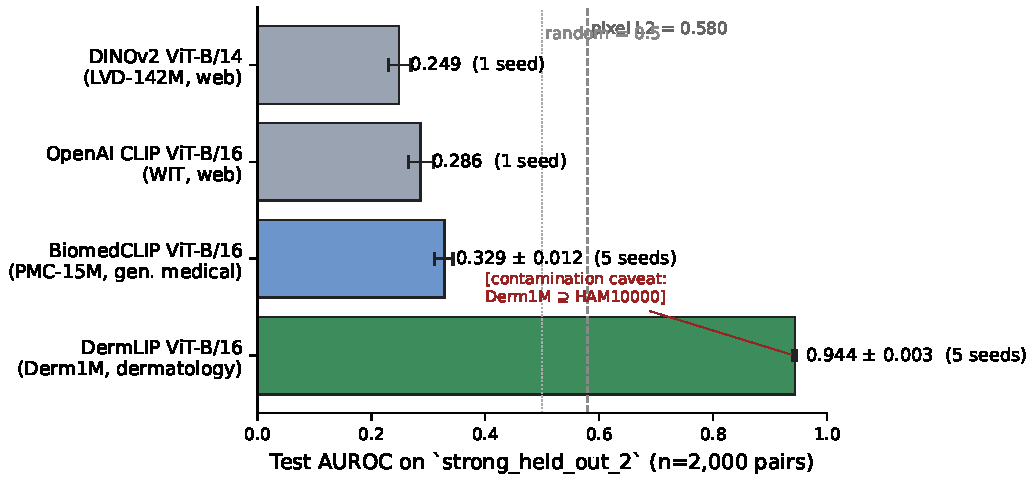
\includegraphics[width=0.85\linewidth]{figures/fig1-cross-backbone-gradient.pdf}
\caption{Test $\auroc$ on \strongholdtwo\ (the unseen third nuisance family)
under the EXP-004 recipe, across four backbones. Error bars are bootstrap
$95\%$ CIs (single seed) or seed-mean $\pm$ standard deviation across five
seeds where available. Pixel L2 (the strongest cheap baseline at $0.580$) is
shown as a dashed reference line. The DermLIP bar carries the contamination
caveat: HAM10000 image-level overlap in Derm1M cannot be excluded
(Appendix~\ref{app:contamination}), and the experiments reported here cannot
separate dermoscopy-domain transfer from such overlap (\S\ref{sec:followup}).}
\label{fig:cross-backbone-gradient}
\end{figure}

Table~\ref{tab:predictor-optimiser} isolates the predictor $\times$
optimiser axis under frozen DINOv2 ViT-B/14: across linear and MLP
predictors, under SGD and Adam, with train $\auroc$ ranging from
$0.572$ to $0.900$, test $\auroc$ on \strongholdtwo\ stays in
$[0.248, 0.270]$ (a $\pm 0.011$ half-range around the midpoint
$0.259$). Scaffold capacity is not the bottleneck.

% Table 2: predictor x optimiser ablation on the EXP-004 proxy under frozen DINOv2 ViT-B/14.
% Source: locked-numbers.json runs exp004_dinov2_linear, exp005_dinov2_mlp_sgd, exp006a_dinov2_mlp_adam.
\begin{table}[h]
\centering
\small
\setlength{\tabcolsep}{6pt}
\begin{tabular}{@{}llrrrr@{}}
\toprule
Run & Predictor & Optimiser & Train $\auroc$ & Test $\auroc$ & 95\% CI \\
\midrule
EXP-004  & linear (identity warm-start)        & SGD  & $0.900$ & $0.249$ & $[0.230, 0.270]$ \\
EXP-005  & 2-layer ID-residual MLP (under-fit) & SGD  & $0.572$ & $0.270$ & $[0.249, 0.293]$ \\
EXP-006a & 2-layer ID-residual MLP (fit)       & Adam & $0.893$ & $0.248$ & $[0.228, 0.269]$ \\
\bottomrule
\end{tabular}
\caption{Predictor $\times$ optimiser ablation under frozen DINOv2
ViT-B/14 on the EXP-004 proxy. Across two predictor classes (linear vs
MLP) and two optimisers (SGD vs Adam), train $\auroc$ ranges from
$0.572$ (under-fit MLP) to $0.900$ (linear) but test $\auroc$ on
\strongholdtwo\ stays in a $\pm 0.011$ band around $0.255$. Scaffold
capacity does not move the held-out-family floor.}
\label{tab:predictor-optimiser}
\end{table}


Table~\ref{tab:seed-sweep} reports the seed sweep on the two
contamination-relevant configurations. Both headline numbers are
seed-stable; the partition gradient is robust to seed variance.

% Table 3: seed sweep on EXP-007 (DermLIP) and EXP-008 (BiomedCLIP).
% Source: docs/experiments/EXP-007-008-seed-sweep-summary.md sections 2--4.
\begin{table}[h]
\centering
\small
\setlength{\tabcolsep}{5pt}
\begin{tabular}{@{}llcrcc@{}}
\toprule
Run & Backbone & $n$ seeds & Test $\auroc$ (mean $\pm$ sd) & Range & 95\% CI[mean] \\
\midrule
EXP-007 & DermLIP B/16    & $5$ & $0.9435 \pm 0.0029$ & $[0.939, 0.947]$ & $[0.941, 0.946]$ \\
EXP-008 & BiomedCLIP B/16 & $5$ & $0.3286 \pm 0.0120$ & $[0.312, 0.344]$ & $[0.318, 0.339]$ \\
\bottomrule
\end{tabular}
\caption{Seed sweep on EXP-007 and EXP-008. Five seeds per
configuration. Both headlines are seed-stable; the seed-mean
pretraining-data gradient (web $0.286 <$ general-medical $0.329 <$
dermoscopy $0.944$) survives. The $\sim$$4\times$ ratio between the two
seed standard deviations is consistent with the high-$\auroc$ DermLIP
regime saturating predictor parameters more reproducibly than the
partial-fit BiomedCLIP regime.}
\label{tab:seed-sweep}
\end{table}


Figure~\ref{fig:train-vs-test-scatter} plots train versus test $\auroc$
for each primary-tier run. The DINOv2 and CLIP runs cluster in the
top-right / bottom-right region (high train, low test) --- a sharp
generalisation gap. EXP-005 sits low on both axes (the under-fit MLP
that barely departed from identity). The DermLIP point is the only one
on the diagonal; BiomedCLIP fits training but does not transfer.

\begin{figure}[h]
\centering
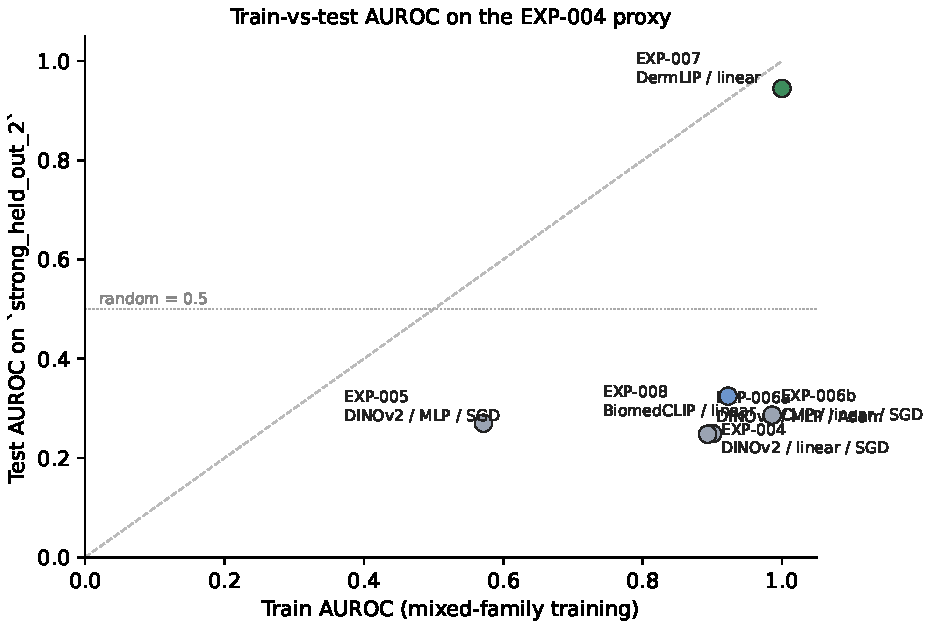
\includegraphics[width=0.78\linewidth]{figures/fig2-train-vs-test-scatter.pdf}
\caption{Train versus test $\auroc$ for each primary-tier run on the
EXP-004 proxy. The dashed diagonal is $\mathrm{train} = \mathrm{test}$;
the dotted horizontal is the random baseline at $0.5$. DermLIP is the
only configuration whose test $\auroc$ tracks training; the four
natural-image configurations sit in the inverted band below the random
line.}
\label{fig:train-vs-test-scatter}
\end{figure}

Figure~\ref{fig:pair-score-histograms} shows the test-split pair-score
distributions for the three CLIP-architecture backbones. The
predictor's score is the cosine distance between its predicted target
and the observed target, so a correctly oriented predictor places
\emph{stable}-pair scores below \emph{changing}-pair scores. CLIP and
BiomedCLIP exhibit the inverted ordering --- stable mean above changing
mean by $0.049$ and $0.034$ respectively --- while DermLIP separates
them by $+0.111$ in the correct direction. The structural inversion
visible here is the mechanism that holds test $\auroc$ to
$0.25$--$0.33$ across natural-image and general-medical pretraining
rather than at chance.

\begin{figure}[h]
\centering
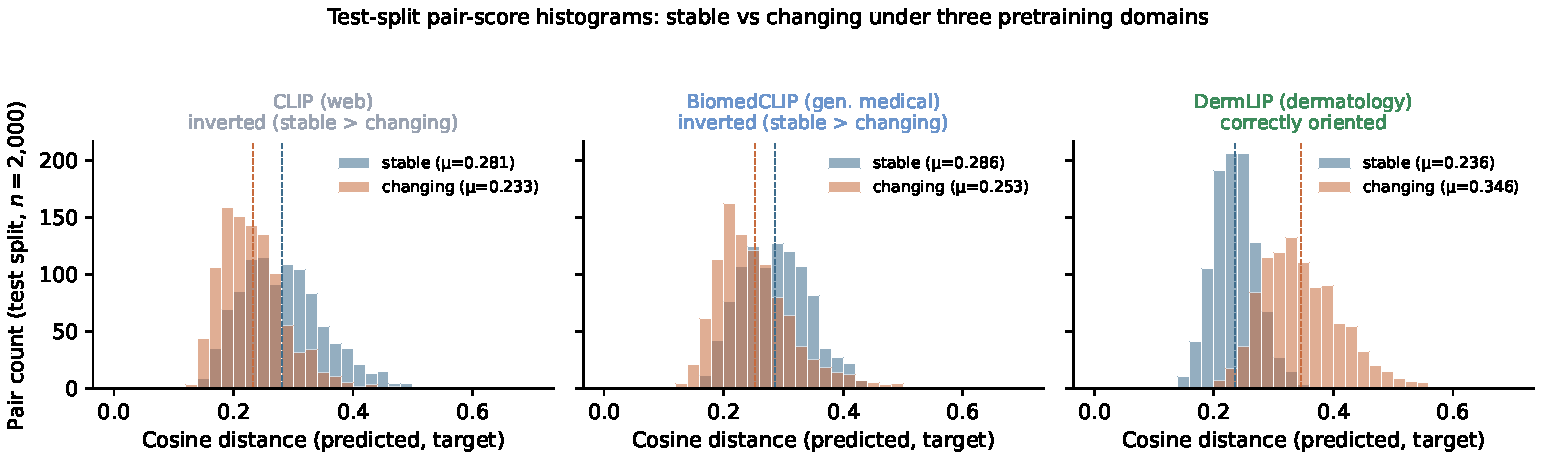
\includegraphics[width=0.98\linewidth]{figures/fig3-pair-score-histograms.pdf}
\caption{Test-split pair-score histograms (cosine distance between the
predictor's predicted target and the observed target) under three
pretraining-data domains, holding architecture (ViT-B/16) and predictor
(linear) constant. Vertical dashed lines mark per-class means. Stable
pairs should lie below changing pairs; the CLIP and BiomedCLIP panels
show the inversion that pulls test $\auroc$ below random, while the
DermLIP panel separates the two classes by $+0.111$ in the correct
direction.}
\label{fig:pair-score-histograms}
\end{figure}

\section{Analysis and discussion}
\label{sec:analysis}

\subsection{Why the inversion is below random rather than at chance}
\label{sec:analysis:inversion}

The below-random orientation of test $\auroc$ under frozen natural-image
backbones is not noise but a structured failure: the linear predictor learns
a direction $w \in \mathbb{R}^{d}$ that encodes ``stable under
$\{\strongfam, \strongholdone\}$'' as small $\langle w, z_{t} - z_{c} \rangle$,
and this direction extrapolates with the \emph{opposite} sign when the unseen
family \strongholdtwo\ rotates the latent geometry the other way. Because the
third family's nuisance is operation-disjoint from the training families, the
rotation does not partially align --- it anti-aligns. Figure~\ref{fig:pair-score-histograms}
shows this structure directly: under frozen OpenAI CLIP, the test-split
stable-pair mean cosine distance ($0.281$) sits \emph{above} the
changing-pair mean ($0.233$), a $-0.049$ inversion gap. Under
BiomedCLIP, the gap narrows to $-0.034$. Under DermLIP, the ordering
flips to the correct direction with a $+0.111$ gap (stable
$0.236$, changing $0.346$). The natural-image inversion is large enough
relative to the within-class spread that $\auroc$ sits in the
$0.25$--$0.29$ band rather than at chance.

\subsection{Why DermLIP transfers under this scaffold and BiomedCLIP doesn't}
\label{sec:analysis:dermlip-vs-biomedclip}

The $+0.66$ $\auroc$ swing from EXP-006b (OpenAI CLIP) to EXP-007 (DermLIP)
cannot be explained by architecture, scaffold, or optimiser: all three are
held byte-identical. The plausible mechanistic accounts are
\begin{enumerate}[label=(\roman*)]
\item DermLIP's CLIP loss over $\sim$1\,M dermatology image-text pairs has
      organised the embedding space such that a single linear direction
      captures stable-pair similarity across all three nuisance families
      uniformly, including \strongholdtwo; or
\item DermLIP saw the HAM10000 raw images during pretraining and its
      embedding space is well-fit to HAM10000 lesion identity in a way that
      survives the synthetic post-hoc nuisance.
\end{enumerate}
EXP-008 rules out a third candidate --- ``any medical-image pretraining'' ---
by showing that BiomedCLIP, trained on $\sim$15\,M PMC-15M figure-caption
pairs without HAM10000, lifts test $\auroc$ by only $+0.04$ over web CLIP.
EXP-008 cannot, however, choose between (i) and (ii). EXP-009 (a
non-HAM10000 dermoscopy SSL pretrain, \S\ref{sec:followup}) is the
experiment that would.

\subsection{Loss versus AUROC}
\label{sec:analysis:loss-vs-auroc}

MSE loss delta does not predict train $\auroc$ across optimisers. From
the per-run training reports
(\texttt{<run\_id>/artifacts/reports/jepa\_training\_report.json} on the
run archive), EXP-006a (Adam, MLP) reduces train MSE by $\sim$$3.3\%$
and reaches train $\auroc = 0.893$, while EXP-004 (SGD, linear) reduces
train MSE by $\sim$$13\%$ and reaches train $\auroc = 0.900$. The
optimisers move the predictor's function very differently per unit of
L2-loss reduction in $768$-d normalised space. Reporting both metrics is
essential, and headline-$\auroc$ comparisons should not be replaced by
loss-only comparisons.

\subsection{What is not yet claimed}
\label{sec:analysis:non-claim}

We do not claim that frozen DermLIP ``solves'' the proxy in a transfer
sense. We claim that frozen DermLIP plus a linear scaffold reaches
$\auroc = 0.944 \pm 0.003$ on \strongholdtwo\ under the specific evaluation
protocol of \S\ref{sec:method}, with HAM10000 contamination unpartitioned.
The result is consistent with two hypotheses --- dermoscopy-domain transfer
and HAM10000 image-level overlap during DermLIP pretraining --- and EXP-009
is required to choose between them. The BiomedCLIP partition rules out only
the broader ``any medical-image pretraining is sufficient'' alternative.

\section{Candidate follow-up: EXP-009}
\label{sec:followup}

We sketch one natural candidate experiment that, if eventually run,
would partition the two hypotheses behind the DermLIP positive. We
present the design now to invite feedback on whether this is the right
follow-up before we (or anyone else) invests the engineering effort
required to run it.

\subsection{The partition question}
The DermLIP positive in EXP-007 ($\auroc = 0.944 \pm 0.003$) is consistent
with two distinct hypotheses. Either DermLIP's dermoscopy-domain pretraining
on Derm1M's non-HAM10000 fraction has aligned nuisance directions across the
three families and that alignment generalises to \strongholdtwo, or DermLIP
saw HAM10000 raw images during pretraining and the embedding space is
well-fit to HAM10000 lesion identity in a way that survives our synthetic
nuisance. EXP-008's BiomedCLIP partition rules out only the broader ``any
medical-image pretraining'' alternative. The dermoscopy-vs-HAM10000
distinction remains open.

\subsection{EXP-009 design}
Self-pretrain a DINOv2 ViT-B/14 encoder on a non-HAM10000 dermoscopy
corpus assembled from ISIC archives minus the HAM10000 split, DermNet,
DermQuest, BCN20000 \citep{combalia2019bcn20000} non-HAM10000 components, and
similar publicly available dermoscopy and clinical-skin sources. Run a short
JEPA-style or masked-image-modelling objective (target: $\sim$20 epochs,
$\sim$200\,k steps), then re-run the EXP-004 recipe on top with the linear
predictor.

\subsection{Decision table}
Table~\ref{tab:exp009-decision} maps the EXP-009 test-$\auroc$ band to a
revision of the paper's claim.

\begin{table}[h]
\centering
\small
\setlength{\tabcolsep}{4pt}
\begin{tabular}{@{}lp{0.32\linewidth}p{0.40\linewidth}@{}}
\toprule
EXP-009 test $\auroc$ & Interpretation & Effect on the paper claim \\
\midrule
$\geq 0.85$    & Dermoscopy-domain transfer is sufficient. & Headline survives; caveat downgrades to ``verified.'' \\
$0.50$--$0.80$ & Partial transfer; mixed contribution. & Claim becomes ``domain helps, dataset overlap helps more.'' \\
$0.30$--$0.50$ & HAM10000 overlap drove EXP-007. & Claim narrows to ``frozen-backbone JEPA unlocks when the backbone has seen the eval dataset.'' \\
\bottomrule
\end{tabular}
\caption{Three EXP-009 outcome bands on \strongholdtwo\ and the
corresponding revision of the paper's claim. Committing this mapping up
front would prevent post-hoc re-interpretation of the experiment.}
\label{tab:exp009-decision}
\end{table}

\subsection{Why we share the design before running it}
Corpus assembly is multi-week: provenance audit on every ISIC component
to confirm HAM10000 exclusion, SSL pretrain compute on a non-trivial
GPU budget, and a pretrain-quality check on a held-out HAM10000 split.
Releasing the methodology and the nine-run arc at this stage is
intentional --- the paper seeks community feedback on the proxy-task
design and on whether this partition is the right follow-up before
anyone (including us) commits to the build. Whether EXP-009, a
different partition, or no follow-up at all is the right next step
depends on that feedback.

\subsection{Feedback we are seeking}
\begin{enumerate}[leftmargin=2em]
\item Is the proxy-task design (three deterministic nuisance families with
      operation-level disjointness, train-on-two / evaluate-on-third) a
      reasonable test of frozen-backbone generalisation, or is a different
      construction more informative?
\item Is the proposed partition (a non-HAM10000 dermoscopy SSL pretrain) the
      right one, or would a different partition (e.g.\ a dermoscopy-text-only
      retrieval probe over DermLIP, or a fine-tuning-on-HAM10000 ablation of
      a known-non-contaminated backbone) be more informative?
\item What other follow-ups would matter for the next stage --- different
      architecture classes, real same-lesion-over-time data, or a different
      evaluation metric?
\item Are there pre-trained backbones in the public literature that would be
      cleaner partition points than the ones we have used?
\end{enumerate}

\section{Limitations}
\label{sec:limitations}

\begin{enumerate}[leftmargin=2em]
\item \textbf{Pretraining contamination is unpartitioned.} The DermLIP
      positive cannot be attributed to dermoscopy-domain transfer with the
      experiments reported here. EXP-009 (\S\ref{sec:followup}) is the
      partition experiment that addresses this; until it runs, the headline
      should be read as ``frozen DermLIP plus a linear scaffold reaches
      $\auroc = 0.944$ under the conditions of \S\ref{sec:method}, with
      HAM10000 contamination unpartitioned'' rather than as a transfer
      claim.
\item \textbf{Synthetic nuisance.} The three families are deterministic
      operations on PIL images. Real-world dermoscopic acquisition
      variability is more complex; the proxy is methodological and is
      identified as such.
\item \textbf{Single-architecture comparison.} All four backbones in the
      cross-backbone gradient are ViT-B/16-class (CLIP-architecture for the
      three CLIP-based ones, ViT-B/14 for DINOv2). Other architectures ---
      DINOv2 self-distillation on different capacity tiers, SigLIP,
      transformer-only image backbones --- are unprobed. Future work should
      vary architecture-class as a separate axis.
\item \textbf{Single dataset.} HAM10000 is the only evaluation corpus.
      ISIC archive components and PAD-UFES-20 are unprobed in this work
      and are candidates for v2 experiments and for the EXP-009 corpus.
\item \textbf{HAM10000 is cross-sectional.} The dataset has no real
      same-lesion-over-time pairs; the longitudinal proxy is synthetic
      throughout. Validating the methodology on a real longitudinal
      dataset (e.g.\ ISIC 2020's serial-imaging metadata) is an explicit
      next-stage follow-up.
\item \textbf{Single scaffold class on the dermoscopy backbone.} The MLP
      ablation (EXP-005, EXP-006a) was run only on DINOv2; an MLP-on-DermLIP
      run was not performed. Predicted to land at or above EXP-007's $0.944$
      since the linear scaffold already saturates training, but unverified.
\end{enumerate}

\section{Conclusion}
\label{sec:conclusion}

We have characterised when frozen-backbone JEPA-style probes fail and when
they succeed under a leakage-controlled, three-family-disjoint nuisance
design on HAM10000. Across four frozen-natural-image configurations
spanning two backbones, two predictor scaffolds, and two optimisers
(the four cells are listed in Appendix~\ref{app:per-run}; we did not
run the full $2 \times 2 \times 2$ factorial), test $\auroc$ on the
held-out third nuisance family inverts below random. Frozen general-
medical pretraining (BiomedCLIP, PMC-15M scientific-article figures,
with no documented raw HAM10000/ISIC archive ingestion) lifts test
$\auroc$ by only $+0.04$. Frozen dermoscopy-pretrained DermLIP reaches test $\auroc = 0.944 \pm 0.003$
across $5$ seeds --- the only above-random result on \strongholdtwo\ among
the six runs that evaluate on it --- but under
a pretraining corpus for which HAM10000 image-level overlap is confirmed (at
small, lower-bounded scale) by a perceptual-hash audit. The methodology,
the configurations, and the run archive are released. We do not claim to have
validated or invalidated the underlying thesis at this stage; we have
characterised a sharp failure mode of the natural-image and general-medical
configurations, observed one positive configuration whose attribution is
unresolved, and sketched one candidate partition experiment (EXP-009)
that, if eventually run, could resolve it. Feedback on the proxy-task
design and on whether this partition is the right next step is the
central purpose of this preliminary release.


\bibliographystyle{plainnat}
\bibliography{refs}

\appendix
\section{Per-run details}
\label{app:per-run}

This appendix re-states the nine-run sequence and the ten-run seed
sweep one entry at a time, anchored on the run identifier so that
readers can navigate from a quoted number to the run-archive folder and
back. Headline numbers therefore overlap with \S\ref{sec:experimental-sequence};
the unique content here is the run-ID, the train$\to$test gap, and any
run-specific anomaly. Each run has a self-contained report at
\path{docs/experiments/EXP-NNN-...md} in the source repository, and
each run's \path{manifest.json}, \path{embeddings/}, \path{metrics.json},
\path{baseline_metrics.json}, \path{config.yaml}, \path{model_card.md},
and \path{logs/} subtree are mirrored under \runarchive\ at
\texttt{<run\_id>/}.

\subsection{EXP-001 --- ceiling sanity}
\label{app:per-run:exp001}
\texttt{ham10000-hf-dinov2-primary-v1}. DINOv2 ViT-B/14, linear, SGD;
mild matched-family nuisance. Train/val/test $\auroc \approx 1.000$ across
every dense baseline and the predictor. Diagnoses the proxy as too easy
and motivates the harder constructions in EXP-002 onward.

\subsection{EXP-002 --- hardened proxy, matched evaluation}
\label{app:per-run:exp002}
\texttt{ham10000-hf-dinov2-exp002-v1}. \strongfam\ on both train and test
splits. Linear-on-DINOv2 reaches test $\auroc = 0.920$, $+0.269$ above
DINOv2 ViT-S/14 raw cosine ($0.652$) with non-overlapping bootstrap CIs.
The ``predict-in-latent-space beats cheap baselines'' claim holds when
the test nuisance distribution matches training.

\subsection{EXP-003 --- one-family-held-out evaluation}
\label{app:per-run:exp003}
\texttt{ham10000-hf-dinov2-exp003-v1}. Train on \strongfam, evaluate on
\strongholdone. Test $\auroc$ falls to $0.680$; SSIM distance becomes the
strongest baseline at $0.961$. The matched-eval delta does not transfer to
a single disjoint nuisance family.

\subsection{EXP-004 --- mixed-family training, third-family evaluation}
\label{app:per-run:exp004}
\path{ham10000-hf-dinov2-exp004-v1}. Train stable pairs rotate between
\strongfam\ and \strongholdone; evaluation on \strongholdtwo. Test
$\auroc = 0.249$ [$0.230, 0.270$]; below-random inversion. Pixel L2
($0.580$) is the strongest baseline. This run defines the canonical
``EXP-004 proxy'' used by every subsequent backbone-ablation run.

\subsection{EXP-005 --- 2-layer identity-residual MLP under SGD}
\label{app:per-run:exp005}
\texttt{ham10000-hf-dinov2-exp005-v1}. Same proxy as EXP-004; replace the
linear predictor with the MLP variant under EXP-002's SGD recipe (LR
$3\!\times\!10^{-2}$, weight decay $10^{-3}$). Train $\auroc = 0.572$
(under-fit; the MLP departs only mildly from identity), test
$\auroc = 0.270$. The scaffold-capacity hypothesis is partially tested
but the MLP has barely moved off the identity init.

\subsection{EXP-006a --- MLP under Adam}
\label{app:per-run:exp006a}
\texttt{ham10000-hf-dinov2-exp006a-v1}. Same MLP as EXP-005 but Adam at
LR $10^{-3}$, decoupled weight decay $10^{-4}$. The optimiser change lets
the MLP fit: train $\auroc = 0.893$, close to EXP-004 linear's $0.900$.
Test $\auroc = 0.248$ [$0.228, 0.269$] --- within a single bootstrap CI of
EXP-004 linear's $0.249$ and below the raw DINOv2 ViT-B/14 cosine baseline
of $0.274$. The properly-fit MLP does not move the held-out-family test
$\auroc$ off the linear-predictor value.

\subsection{EXP-006b --- OpenAI CLIP ViT-B/16}
\label{app:per-run:exp006b}
\texttt{ham10000-hf-clip-exp006b-v1}. EXP-004 recipe with the backbone
swapped from DINOv2 ViT-B/14 to OpenAI CLIP ViT-B/16. Test $\auroc =
0.286$ [$0.265, 0.310$], overlapping bootstrap CIs with EXP-004's $0.249$.
The below-random inversion is not DINOv2-specific. Train $\auroc = 0.986$;
the train$\to$test drop is $-0.70$.

\subsection{EXP-007 --- DermLIP ViT-B/16}
\label{app:per-run:exp007}
\texttt{ham10000-hf-dermlip-exp007-v1}. EXP-004 recipe with the backbone
swapped from OpenAI CLIP to DermLIP. Test $\auroc = 0.945$ [$0.935, 0.954$]
on the original seed; first above-random result on \strongholdtwo\ since
EXP-002 (and the only one across nine primary-tier runs). The
contamination caveat is introduced here: Derm1M's data card does not
publish a per-source breakdown, but HAM10000 raw images are almost
certainly included (Appendix~\ref{app:contamination}).

\subsection{EXP-008 --- BiomedCLIP ViT-B/16}
\label{app:per-run:exp008}
\texttt{ham10000-hf-biomedclip-exp008-v1}. EXP-004 recipe with the
backbone swapped to BiomedCLIP (PMC-15M, no HAM10000). Test $\auroc =
0.325$ [$0.303, 0.349$]. The web $\to$ general-medical step contributes
$+0.04$; the general-medical $\to$ dermoscopy step contributes $+0.62$.
EXP-008 rules out ``any medical-image pretraining'' as sufficient but
does not partition dermoscopy-domain transfer from HAM10000 image-level
overlap.

\subsection{Seed sweep on EXP-007 and EXP-008}
\label{app:per-run:seed-sweep}
Five seeds per configuration, ten runs total.
\texttt{...-dermlip-exp007-seed-\{1,2,3,4\}-v1} and
\texttt{...-biomedclip-exp008-seed-\{1,2,3,4\}-v1} alongside the
canonical seed-$20260422$ runs. DermLIP test $\auroc = 0.9435 \pm 0.0029$
(range $0.9392$--$0.9470$, $95\%$ CI[mean] $[0.9409, 0.9461]$); BiomedCLIP
test $\auroc = 0.3286 \pm 0.0120$ (range $0.3119$--$0.3436$, $95\%$
CI[mean] $[0.3181, 0.3391]$). The seed-to-seed sd ratio
($0.012 / 0.003 \approx 4\times$) is consistent with the high-$\auroc$
DermLIP regime saturating predictor parameters more reproducibly than the
partial-fit BiomedCLIP regime. The pretraining-data gradient (web $0.286$
$<$ general-medical $0.329$ $<$ dermoscopy $0.944$) survives seed variance.

\section{Hyperparameters}
\label{app:hyperparameters}

Table~\ref{tab:hyperparameters} lists the predictor hyperparameters used
in every primary-tier run. Values are stable across all nine runs (and
the ten seed-sweep runs); only the predictor type, the optimiser, and
the backbone are varied between runs. The full per-run configurations
are committed under \texttt{configs/data/} and mirrored alongside every
run as \texttt{<run\_id>/config.yaml}.

\begin{table}[h]
\centering
\small
\setlength{\tabcolsep}{4pt}
\begin{tabular}{@{}lp{0.36\linewidth}p{0.42\linewidth}@{}}
\toprule
Setting & Linear predictor & 2-layer identity-residual MLP \\
\midrule
Architecture        & $g_{\theta}(z) = Wz + b$ & $g_{\theta}(z) = z + W_{2}\,\mathrm{ReLU}(W_{1}z + b_{1}) + b_{2}$ \\
Hidden dim          & ---       & $512$ \\
Init $W$ / $W_{1}$  & $I + \epsilon$, $\epsilon_{ij} \sim \mathcal{N}(0, 0.005^{2})$ & Kaiming-uniform \\
Init $W_{2}$        & ---       & zero ($g_{\theta} = \mathrm{id}$ at step $0$) \\
Init biases         & zero      & zero \\
Optimiser           & SGD       & SGD (EXP-005) / Adam (EXP-006a) \\
Learning rate       & $3\!\times\!10^{-2}$ & $3\!\times\!10^{-2}$ / $10^{-3}$ \\
Weight decay        & $10^{-3}$ on $(W - I)$ & $10^{-3}$ on $W_{1}, W_{2}$ / $10^{-4}$ decoupled \\
Batch size          & $128$     & $128$ \\
Epochs              & $200$     & $200$ \\
Grad. clipping      & none      & none \\
LR schedule         & constant  & constant \\
Loss                & L2-MSE on stable pairs (eq.~\ref{eq:loss}) & L2-MSE on stable pairs \\
Bootstrap           & $1{,}000$ resamples, per-pair & $1{,}000$ resamples, per-pair \\
Seed (default)      & $20260422$ & $20260422$ \\
\bottomrule
\end{tabular}
\caption{Predictor hyperparameters. Every other knob (split fractions,
seed, pair counts, augmentation parameters) is held constant across all
nine primary-tier runs and across the ten seed-sweep runs.}
\label{tab:hyperparameters}
\end{table}

\paragraph{Embedding precondition.} Backbone outputs are L2-normalised
before entering the predictor (eq.~\ref{eq:loss}). Predictor outputs are
L2-normalised before the cosine-distance score
(eq.~\ref{eq:score}). No batch normalisation, dropout, or stochastic
depth is used inside the predictor.

\paragraph{Backbone configurations.} All backbones run in inference mode
(\texttt{eval()}, no gradient). Embedding dimensions: DINOv2 ViT-B/14
$d = 768$; OpenAI CLIP ViT-B/16 $d = 512$; DermLIP ViT-B/16 $d = 512$;
BiomedCLIP ViT-B/16 $d = 512$. The predictor input/output dimensionality
matches the backbone output and is set automatically from each backbone's
configured embedding size.

\section{Nuisance-family operation specifications}
\label{app:nuisance-operations}

The three nuisance families in \S\ref{sec:method:nuisance} are
implemented in \path{src/derma_jepa/public_data.py}: \strongfam\ at
line 751 (\path{_apply_strong_nuisance}), \strongholdone\ at line 829
(\path{_apply_strong_held_out_nuisance}), and \strongholdtwo\ at line
494 (\path{_apply_strong_held_out_2_nuisance}). Each function takes a
PIL image, a per-pair index, and a NumPy \texttt{Generator}, applies
the operations below in the listed order, and returns the
nuisance-perturbed image alongside a recipe dictionary recording the
sampled parameter values.

\subsection*{\strongfam}
Photometric, geometric, and sensor-noise perturbations that model
ordinary acquisition variability.
\begin{itemize}
\item Brightness, contrast, and saturation jitter applied independently:
      each scaled by $u \sim \mathrm{Uniform}(0.6, 1.4)$ via PIL
      \texttt{ImageEnhance}.
\item Affine transform: rotation $\theta \sim \mathrm{Uniform}(-15^{\circ}, 15^{\circ})$,
      isotropic scale $s \sim \mathrm{Uniform}(0.82, 1.00)$, translation
      $(t_{x}, t_{y}) \sim \mathrm{Uniform}(-0.05, 0.05)^{2}$ in image-fraction units.
\item Horizontal flip with probability $0.5$.
\item Gaussian blur with radius $r \sim \mathrm{Uniform}(0.5, 1.5)$\,px.
\item Additive Gaussian noise with $\sigma \sim \mathrm{Uniform}(0, 8)$
      on the $0$--$255$ scale.
\item JPEG round-trip at quality $q \sim \mathrm{Uniform}\{45, \dots, 70\}$.
\end{itemize}

\subsection*{\strongholdone}
Disjoint operation set: HSV colour rotation, posterisation, sharpening,
motion blur, occlusion, and aggressive JPEG compression. No transform
type overlaps with \strongfam.
\begin{itemize}
\item HSV hue rotation by $\Delta h \sim \mathrm{Uniform}(-12^{\circ}, 12^{\circ})$.
\item Posterise to $b \sim \mathrm{Uniform}\{4, 5, 6\}$ bits per channel.
\item Unsharp-mask sharpen with PIL \texttt{ImageFilter.UnsharpMask}
      (radius $2$, percent $\sim \mathrm{Uniform}(120, 200)$, threshold $3$).
\item Motion blur with a linear kernel of length $k \sim \mathrm{Uniform}\{5, \dots, 15\}$\,px,
      orientation chosen uniformly from \{vertical, horizontal\}.
\item Random rectangular erasing covering
      $\alpha \sim \mathrm{Uniform}(0.06, 0.18)$ of the image area, fill
      colour sampled per call from $\{0, 128, 255\}$.
\item JPEG round-trip at quality $q \sim \mathrm{Uniform}\{20, \dots, 40\}$.
\end{itemize}

\subsection*{\strongholdtwo}
Disjoint operation set: gamma, colour-temperature, vignette,
salt-and-pepper noise, and high-quality JPEG. No transform type overlaps
with \strongfam\ or \strongholdone.
\begin{itemize}
\item Gamma correction with $\gamma \sim \mathrm{Uniform}(0.6, 1.6)$
      (non-linear, distinct from contrast).
\item Colour-temperature shift: scale R by
      $T \sim \mathrm{Uniform}(0.85, 1.15)$ and divide B by $T$.
\item Radial vignette with cos$^{2}$ falloff at strength
      $v \sim \mathrm{Uniform}(0.25, 0.55)$ from image centre.
\item Salt-and-pepper impulse noise covering
      $\rho \sim \mathrm{Uniform}(0.005, 0.025)$ of pixels with value
      drawn uniformly from $\{0, 255\}$.
\item JPEG round-trip at quality $q \sim \mathrm{Uniform}\{80, \dots, 95\}$
      (distinct from \strongfam's $45$--$70$ and \strongholdone's $20$--$40$).
\end{itemize}

\paragraph{Disjointness.} The three operation sets share no transform
type --- a property enforced by inspection of the function bodies and
re-checked in the code review for every new family proposed. JPEG
quality ranges are chosen non-overlapping so that the post-pipeline
compression artefact is family-distinguishable. The composite
augmentation pipeline is deterministic in the per-pair seed: the same
seed reproduces byte-identical perturbed images, which is exploited by
the verification harness in \texttt{tests/test\_public\_data\_pipeline.py}.

\section{Bootstrap CI protocol}
\label{app:bootstrap-protocol}

Every $\auroc$ in the paper is reported with a $1{,}000$-sample
percentile bootstrap $95\%$ confidence interval. The implementation is
at \path{src/derma_jepa/metrics.py:66}
(\path{bootstrap_auroc_ci}); the unit tests at
\path{tests/test_metrics.py} cover the AUROC point estimate, the
bootstrap CI shape, the equal-error-rate threshold, and the
FPR-at-fixed-TPR computation.

\paragraph{Resampling unit.} The resampling unit is the pair: each
bootstrap sample draws $N$ stable--changing pair indices with
replacement from the $N = 2{,}000$ pairs in a split, recomputes
$\auroc$ on the resampled set, and records the value. The $2.5\%$ and
$97.5\%$ percentiles of the $1{,}000$ resampled $\auroc$ values define
the reported CI. Pair-level resampling matches the unit at which the
score $s$ is computed (eq.~\ref{eq:score}); it does not stratify by
diagnosis or by anatomical site.

\paragraph{Determinism.} The bootstrap RNG is seeded from the same
project seed used for split assignment, predictor initialisation, and
pair generation. Re-running a configuration with the same seed
reproduces byte-identical CIs.

\paragraph{Seed-mean CIs.} For the EXP-007 and EXP-008 seed sweeps
(\S\ref{app:per-run:seed-sweep}), the reported $\pm$ values are
unbiased standard deviations across the five seed-mean $\auroc$
estimates; the reported ``$95\%$ CI[mean]'' is the seed-mean point
estimate plus and minus $1.96$ times the seed-mean standard error
($\sigma / \sqrt{n}$ with $n = 5$). These intervals quantify seed
variance and are distinct from the per-pair bootstrap CIs reported on a
single seed.

\paragraph{Companion metrics.} Alongside $\auroc$, every run reports
AUPRC, the equal-error-rate threshold, and the false-positive rate at a
fixed true-positive rate of $0.8$. Each is bootstrapped under the same
protocol. AUPRC tracks $\auroc$ rank-monotonically across the nine runs;
EER and FPR-at-TPR add operating-point information that is sensitive to
the train$\to$test score-distribution shift discussed in
\S\ref{sec:analysis:inversion}. Per-run values are mirrored at
\texttt{<run\_id>/metrics.json} under \runarchive.

% Appendix stub --- draft from docs/paper/OUTLINE.md \S8 and the per-run reports.
\section{Representation-health checks}
\label{app:representation-health}
\todo[inline]{Draft from the corresponding OUTLINE \S8 pointer plus the relevant sources under \texttt{docs/experiments/} or \texttt{src/derma\_jepa/}.}

\section{Compute budget}
\label{app:compute-budget}

Every primary-tier run executes on a single NVIDIA A10G 24~GB via
Hugging Face Jobs (\texttt{a10g-large}). The wall-clock breakdown for
the canonical EXP-004 recipe ($\sim$85~min end-to-end) is approximately:

\begin{itemize}
\item Manifest build, deterministic-augmentation pair generation, and
      data-audit checks: $\sim$10~min.
\item Backbone embedding export over $6{,}000$ pairs ($\times 2$ sides):
      $\sim$10~min for ViT-B/14--B/16 backbones.
\item Cheap-baseline evaluation (pixel L2, SSIM, raw cosine): $\sim$5~min.
\item Predictor training ($200$ epochs, batch $128$, $\sim$8 steps per
      epoch): $\sim$50~min for the linear predictor; the MLP predictor
      runs in the same envelope.
\item Bootstrap CIs, representation-health checks, report writing,
      run-archive upload: $\sim$10~min.
\end{itemize}

The MLP-on-DINOv2 runs (EXP-005 and EXP-006a) take $\sim$105~min
because the MLP forward/backward is approximately twice the linear
predictor's. The DermLIP and BiomedCLIP runs sit in the same
$\sim$85-minute envelope as the linear DINOv2 and CLIP runs: backbone
forward dominates only the embedding-export phase, and once
embeddings are cached, predictor training is backbone-independent.

\paragraph{Total for the paper.} Nine primary-tier runs at $\sim$85--105
min each plus eight additional seed-sweep runs at $\sim$85~min each
totals approximately $25$ A10G-hours of compute, plus an additional
$\sim$3~A10G-hours absorbed by two infrastructure-flake re-launches
during the seed-sweep cohort. All accumulated at Hugging Face Jobs
free-tier rates; the launchers are committed under \path{scripts/}
and the pinned dependency versions for the hosted environment are at
\path{scripts/hf_jobs_constraints.txt}.

\paragraph{Reproducibility cost.} Reproducing the entire nine-run arc
plus the seed sweep from a clean checkout requires the same $\sim$28
A10G-hours, plus a one-time HAM10000 download (the source manifest
caches it once). No private data, no local GPU.

% Appendix stub --- draft from docs/paper/OUTLINE.md \S8 and the per-run reports.
\section{Reproducibility checklist}
\label{app:reproducibility-checklist}
\todo[inline]{Draft from the corresponding OUTLINE \S8 pointer plus the relevant sources under \texttt{docs/experiments/} or \texttt{src/derma\_jepa/}.}

\section{Pretraining contamination analysis}
\label{app:contamination}

This appendix is load-bearing for the paper's central claim. It states
the contamination question precisely, lays out the available evidence,
and identifies what EXP-007 / EXP-008 can and cannot conclude from that
evidence.

\subsection{The question}
The EXP-007 result --- frozen DermLIP plus a linear scaffold reaches
test $\auroc = 0.944 \pm 0.003$ on \strongholdtwo\ --- is consistent with
two distinct hypotheses:
\begin{enumerate}[label=(\roman*), leftmargin=2em]
\item \emph{Dermoscopy-domain transfer.} Pretraining on dermatology image-
      text pairs (Derm1M) organises the embedding space such that a
      single linear direction captures stable-pair similarity uniformly
      across the three nuisance families, including the unseen
      \strongholdtwo.
\item \emph{HAM10000 image-level overlap.} Derm1M contains HAM10000 (or
      near-duplicate) images via its uncontrolled literature/web sources,
      so DermLIP's embedding space is well-fit to HAM10000 lesion identity
      in a way that survives our synthetic post-hoc nuisance.
\end{enumerate}
Hypotheses (i) and (ii) are not mutually exclusive: a positive
EXP-009 outcome (\S\ref{sec:followup}) would support (i) being load-bearing;
a low EXP-009 outcome would push the explanation toward (ii).

\subsection{Is HAM10000 in Derm1M?}
Derm1M \citep{yan2025derm1m} names exactly two public datasets as image
sources --- SCIN and MSKCC (an ISIC-archive subset \citep{codella2018isic})
--- and HAM10000 \citep{tschandl2018ham10000} is not among them: in the
Derm1M paper HAM10000 appears only as a downstream evaluation benchmark,
as a comparison row in the related-datasets table, and as a source of
disease \emph{label names} for the standardised taxonomy. At the level of
named sources, HAM10000 is therefore not a constituent of Derm1M, and the
named MSKCC source is a Memorial-Sloan-Kettering ISIC subset contributed by
a different institution than HAM10000's Vienna/Rosendahl images, so it is
unlikely to introduce HAM10000 images directly.

Overlap is nonetheless present through Derm1M's \emph{uncontrolled} sources.
Derm1M documents no deduplication or decontamination against HAM10000 or any
downstream benchmark, and beyond its two named public datasets it
bulk-aggregates PubMed figures, educational video, and social-media
dermatology content, in which HAM10000 --- the most widely reproduced public
dermoscopy dataset --- circulates freely. A perceptual-hash audit of HAM10000
against the (access-gated) Derm1M corpus confirms this: at least
\textbf{13 distinct HAM10000 images}, drawn from at least four PubMed Central
articles, are present in Derm1M's PubMed/literature partition, verified by
agreement across four independent perceptual hashes (pHash, dHash, aHash,
wHash) and by visual inspection (one journal figure alone, PMC9777332, is a
multi-panel montage reproducing roughly five HAM10000 dermoscopy images). The
13 is a lower bound: dermoscopy images collide heavily under any single
perceptual hash, so only multi-hash-plus-visual matches were counted; the
forum and textbook candidates were not all individually verified; and the
$16.6$\,GB YouTube-frame partition was not audited. DermLIP's pretraining was
therefore \emph{not} HAM10000-free. The confirmed scale is small relative to
HAM10000's $10{,}015$ images, which makes wholesale memorisation an unlikely
\emph{sole} explanation of the EXP-007 win, but it does not clear the
confound; the EXP-009 partition (\S\ref{sec:followup}), which holds
``HAM10000 absent'' constant by construction, remains the way to separate
dermoscopy-domain transfer from overlap. Full method and per-article findings
are in the repository's overlap-audit report.

\subsection{What EXP-007 alone can conclude}
EXP-007 demonstrates a $+0.66$ test $\auroc$ swing relative to
EXP-006b (OpenAI CLIP) when the only varied axis is the pretraining
data. EXP-007 alone cannot distinguish (i) from (ii), and the paper
explicitly does not attribute the swing to dermoscopy-domain transfer
on the basis of EXP-007 alone.

\subsection{What EXP-008 adds and what it does not}
EXP-008 introduces a third pretraining-data point: BiomedCLIP's PMC-15M,
which is approximately $15\times$ larger than Derm1M but is composed of
biomedical figure--caption pairs with a very low fraction of
dermoscopy and no documented raw HAM10000/ISIC archive ingestion. The result --- test
$\auroc = 0.329 \pm 0.012$ --- contributes three readings:
\begin{itemize}
\item \textbf{Scale alone is not the explanation.} Fifteen million
      biomedical pairs without documented raw HAM10000/ISIC archive
      ingestion do not unlock the proxy, so the
      EXP-007 win is not attributable to ``more pretraining data,''
      ``more medical pretraining data,'' or any monotonic function of
      pretraining-corpus size.
\item \textbf{General medical pretraining is not the explanation.} The
      $+0.04$ web $\to$ general-medical step is small relative to the
      $+0.62$ general-medical $\to$ dermoscopy step. The unlock is
      localised at the dermoscopy-specific corpus boundary.
\item \textbf{Dermoscopy-vs-HAM10000 remains unresolved.} EXP-008's
      pretraining corpus differs from EXP-007's in two ways
      simultaneously --- domain narrowness and (likely) HAM10000
      overlap (confirmed, small-scale) --- so
      EXP-008 cannot separate the two factors. EXP-009
      (\S\ref{sec:followup}) is designed precisely to break this
      confound by holding ``HAM10000 absent'' constant while varying
      the pretraining-domain narrowness from PMC-15M to dermoscopy.
\end{itemize}

\subsection{Boundary of inference}
The strongest claim the paper makes about the EXP-007 swing is the
following: \emph{under the protocol of \S\ref{sec:method}, varying only
the pretraining-data domain among DermLIP, BiomedCLIP, and OpenAI
CLIP --- holding architecture, predictor, optimiser, hyperparameters,
and data pipeline constant --- produces a $+0.66$ $\auroc$ swing
localised to the dermoscopy-specific corpus.} The claim is a
characterisation of the empirical gradient, not an attribution to
domain transfer. The corresponding negative claim --- ``DermLIP
generalises to \strongholdtwo\ because dermoscopy pretraining unlocks
nuisance invariance'' --- is not made anywhere in the paper.

\section{EXP-009 design (planned)}
\label{app:exp009-design}

This appendix expands the EXP-009 sketch in \S\ref{sec:followup} into the
operational details required to launch the experiment. The design is
committed in advance --- including the decision table mapping outcome
bands to claim revisions --- so the experiment cannot be re-interpreted
post-hoc.

\subsection{Goal}
Self-pretrain a vision encoder on a non-HAM10000 dermoscopy corpus, then
re-run the EXP-004 recipe on top with the linear predictor. The encoder
sees no HAM10000 image during pretraining, so the EXP-007-style positive
on \strongholdtwo\ --- if it appears --- can no longer be attributed to
HAM10000 image-level overlap and must reflect dermoscopy-domain transfer.

\subsection{Pretraining corpus}
Assemble from publicly available dermoscopy / clinical-skin sources, with
provenance audit on every component to confirm HAM10000 exclusion:
\begin{itemize}
\item ISIC archive components other than HAM10000 (BCN20000
      \citep{combalia2019bcn20000}, MSK-1 through MSK-5, UDA, Mednode,
      and similar legacy archives).
\item DermNet NZ and DermQuest-derived public images (clinical, not
      dermoscopic; included to broaden the visual distribution).
\item PAD-UFES-20 and 7-point checklist datasets (each cross-checked
      for HAM10000 overlap by lesion-ID and SHA-256 hash).
\end{itemize}
Provenance audit: every image must carry a source attribution and a
SHA-256 hash. The HAM10000 image-hash set is computed from the source
manifest and excluded by hash; any image whose source attribution is
ambiguous is excluded by default.

\subsection{Pretraining objective}
DINOv2 ViT-B/14 architecture (i.e.\ the same family as the EXP-004
backbone, so any test-$\auroc$ change is attributable to pretraining
data, not architecture), trained for $\sim$20 epochs with a JEPA-style
or masked-image-modelling objective. Hyperparameters target a
$\sim$$200{,}000$-step regime on a $\sim$$8\times$~A10G or
$1\times$~A100 budget. Pretrain-quality is checked by linear-probing on
a held-out HAM10000 split for diagnosis classification --- a sanity
check that the encoder has not overfit to its training distribution.

\subsection{Probe}
After pretraining, the encoder is frozen and the EXP-004 recipe runs on
top: linear predictor with identity warm-start, SGD, weight-decay-on-$(W-I)$,
$200$ epochs, the same lesion-ID splits, the same $1{,}000 + 1{,}000$
pairs per split, the same three-family augmentation pipeline, the same
seed. The only varied axis relative to EXP-004 is the pretraining
data; the only varied axis relative to EXP-007 is HAM10000 inclusion in
that pretraining data.

\subsection{Decision table}
Identical to Table~\ref{tab:exp009-decision} in \S\ref{sec:followup}.
Outcome bands and claim revisions:
\begin{itemize}
\item Test $\auroc \geq 0.85$: dermoscopy-domain transfer is sufficient
      under this scaffold. Headline survives; contamination caveat
      downgrades from ``unpartitioned'' to ``ruled out.''
\item Test $\auroc$ in $[0.50, 0.80]$: partial transfer; both factors
      contribute. Claim becomes ``dermoscopy-domain pretraining helps,
      HAM10000 image overlap helps more.''
\item Test $\auroc$ in $[0.30, 0.50]$: HAM10000 overlap drove EXP-007.
      Claim narrows to ``frozen-backbone JEPA unlocks when the backbone
      has seen the eval dataset, not when it has seen the eval
      domain.''
\end{itemize}

\subsection{Why not run before this preprint}
Three concrete costs gate the launch:
\begin{enumerate}[label=(\arabic*), leftmargin=2em]
\item \emph{Provenance audit.} Confirming HAM10000 exclusion on every
      ISIC component requires a per-image hash check against the
      HAM10000 manifest --- the audit is straightforward but is itself
      a multi-day engineering task before any GPU is spent.
\item \emph{Pretrain compute.} DINOv2 ViT-B/14 pretraining on
      $\sim$$200{,}000$ steps requires a non-trivial GPU budget that is
      not in the free-tier envelope used for the other nine runs.
\item \emph{Pretrain-quality validation.} A weak pretraining run that
      never learns dermoscopy structure would produce a low test
      $\auroc$ that the decision table would mis-attribute to (ii) or
      (iii) when the actual cause is pretrain failure. We need a
      held-out diagnostic to disambiguate.
\end{enumerate}
We share the methodology and the nine-run arc at this stage to invite
feedback on the proxy-task design and on whether the proposed partition
is the right one before committing to the build.


\end{document}
